\documentclass[11pt,a4paper]{article}
			\usepackage[french]{babel}
					
				\usepackage{pifont}  
				\usepackage[utf8x]{inputenc}
				\usepackage[T1]{fontenc} 
				\usepackage{lmodern}			
				\usepackage{fancyhdr}
				\usepackage{textcomp}
				\usepackage{makeidx}
				\usepackage{tabularx}
				\usepackage{multicol}
				\usepackage{multirow}
				\usepackage{longtable}
				\usepackage{color}
				\usepackage{soul}
				\usepackage{boxedminipage}
				\usepackage{shadow}
				\usepackage{framed}			
				\usepackage{array}
				\usepackage{url}
				\usepackage{ragged2e}
				\usepackage{fancybox}
				\newcommand{\cadretitre}[2]{
				  \vspace*{0.8\baselineskip}
				  \begin{center}%
				  \boxput*(0,1){%
					%\colorbox{white}{\Large\textbf{\ #1\ }}%
				  }%
				  {%
					\setlength{\fboxsep}{10pt}%
				    \Ovalbox{\begin{minipage}{.8\linewidth}\begin{center}\Large\sffamily{#2}\end{center}\end{minipage}}}%
				  \end{center}
				  \vspace*{2\baselineskip}
				  }
			
			\makeatletter
			\def\@seccntformat#1{\protect\makebox[0pt][r]{\csname the#1\endcsname\quad}}
			\makeatother

				% Permet d'afficher qqchose à une positin absolue
				\usepackage[absolute]{textpos}
				\setlength{\TPHorizModule}{1cm}
				\setlength{\TPVertModule}{\TPHorizModule}
	
				\usepackage[titles]{tocloft}
				\setlength{\cftbeforesecskip}{0.5ex}
				\setlength{\cftbeforesubsecskip}{0.2ex}
				\addto\captionsfrench{\renewcommand\contentsname{}}
				
				\usepackage[font=scriptsize]{caption}
				
				\usepackage{listings}
\lstdefinestyle{lstverb}
  {
    basicstyle=\footnotesize,
    frameround=tttt, frame=trbl, framerule=0pt, rulecolor=\color{gray},
    lineskip=-1pt,   % pour rapprocher les lignes
    flexiblecolumns, escapechar=\\,
    tabsize=4, extendedchars=true
  }
\lstnewenvironment{Java}[1][]{\lstset{style=lstverb,language=java,#1}}{}
				\ifx\pdfoutput\undefined
					\usepackage{graphicx}
				\else
					\usepackage[pdftex]{graphicx}
				\fi
				\usepackage[a4paper, hyperfigures=true, colorlinks, linkcolor=black, citecolor=blue,urlcolor=blue, pagebackref=true, bookmarks=true, bookmarksopen=true,bookmarksnumbered=true,
                pdfauthor={}, pdftitle={TD Tableaux}, pdfkeywords={TD Tableaux, },pdfpagemode=UseOutlines,pdfpagetransition=Dissolve,nesting=true,
				backref, pdffitwindow=true, bookmarksnumbered=true]{hyperref}
				\usepackage{supertabular}
				\usepackage[table]{xcolor}
				\usepackage{url}
				\usepackage{caption} 
				\setlength{\parskip}{1.3ex plus 0.2ex minus 0.2ex}
				\setlength{\parindent}{0pt}
				
				\makeatletter
				\def\url@leostyle{ \@ifundefined{selectfont}{\def\UrlFont{\sf}}{\def\UrlFont{\footnotesize\ttfamily}}}
				\makeatother
				\urlstyle{leo}
				
				\definecolor{examplecolor}{rgb}{0.156,0.333,0.443}
				\definecolor{definitioncolor}{rgb}{0.709,0.784,0.454}
				\definecolor{exercisecolor}{rgb}{0.49,0.639,0}
				\definecolor{hintcolor}{rgb}{0.941,0.674,0.196}
				\definecolor{tableHeadercolor}{rgb}{0.709,0.784,0.454}
				\definecolor{tablerowAltcolor}{rgb}{.866,.905,.737}
				\definecolor{tablerowAlt2color}{rgb}{.968,.976,.933}
				\definecolor{verylightgray}{rgb}{0.98,0.98,0.98}
				
				\newenvironment{fshaded}{
				\def\FrameCommand{\fcolorbox{framecolor}{shadecolor}}
				\MakeFramed {\FrameRestore}}
				{\endMakeFramed}
				
				\newenvironment{fexample}[1][]{\definecolor{shadecolor}{rgb}{.913,.913,.913}
				\definecolor{framecolor}{rgb}{.156,.333,.443}
				\begin{fshaded}}{\end{fshaded}} 
				
				\newenvironment{fdefinition}{\definecolor{shadecolor}{rgb}{.913,.913,.913}
				\definecolor{framecolor}{rgb}{.709,.784,.454}
				\begin{fshaded}}{\end{fshaded}}
				
				\newenvironment{fexercise}{\definecolor{shadecolor}{rgb}{.913,.913,.913}
				\definecolor{framecolor}{rgb}{.49,.639,0}
				\begin{fshaded}}{\end{fshaded}}
				
				\newenvironment{fhint}{\definecolor{shadecolor}{rgb}{.913,.913,.913}
				\definecolor{framecolor}{rgb}{.941,.674,.196}
				\begin{fshaded}}{\end{fshaded}}	
				
				\newcommand{\PreserveBackslash}[1]{
				\let\temp=\\#1\let\\=\temp
				}
				\let\PBS=\PreserveBackslash
				\newcolumntype{A}{>{\PBS\raggedright\small\hspace{0pt}}X}
				\newcolumntype{L}[1]{>{\PBS\raggedright\small\hspace{0pt}}p{#1}}
				\newcolumntype{R}[1]{>{\PBS\raggedleft\small\hspace{0pt}}p{#1}}
				\newcolumntype{C}[1]{>{\PBS\centering\small\hspace{0pt}}p{#1}}
				
				\makeindex
				
				\title{TD Tableaux}	
			\date{}
			\author{\scriptsize{}}
			\definecolor{light-gray}{gray}{0.8}
			\renewcommand{\headrulewidth}{0pt}
			\fancyhead[L]{
				\footnotesize\textsc{Haute \'Ecole de Bruxelles}\\
	    			\footnotesize\textsc{\'Ecole Sup\'erieure d'Informatique}
			}
			\fancyhead[R]{
				\footnotesize{Bachelor en Informatique}\\
				\footnotesize{Laboratoires Java} - 
			\footnotesize{1\`ere ann\'ee}}
				\fancyfoot[L]{ }
				\fancyfoot[C]{}
				\fancyfoot[R]{\scriptsize{\textcolor{gray}{version 2014-2015 (\today)}}}
				\pagestyle{plain}
				\reversemarginpar
				\usepackage{rotating}						
				\begin{document}
					\begin{textblock}{9}(2,3.2)
						
\includegraphics[width=2cm]{../../../_templates/java/icons/logo-esi}
					\end{textblock}
				
				
				
				
				%\maketitle
				\cadretitre{TD1}{TD Tableaux}
				\thispagestyle{fancy}
        \marginpar{\begin{sideways}
            \begin{minipage}[t]{1cm}
            \begin{tiny}
            
\includegraphics[width=1\linewidth,height=1\textheight,keepaspectratio=true]{../../../_templates/java/icons/cc-gris.jpg}
			\end{tiny}
			\end{minipage}
            \begin{minipage}[b]{19cm}
            \begin{tiny}
            \textcolor{gray}{Distribué sous licence Creative Commons Paternité - Partage à l'Identique 2.0 Belgique 
            (\texttt{http://creativecommons.org/licenses/by-sa/2.0/be/})
			\vspace{-1em}
			\\Les autorisations au-delà du champ de cette licence peuvent être obtenues à 
			\texttt{http://www.heb.be/esi}
			- \texttt{mcodutti@heb.be}
			}\end{tiny}
			\end{minipage}
        \end{sideways}}
            \begin{abstract}
			Voyons ici les tableaux, une structure qui peut contenir plusieurs exemplaires de donn\'ees similaires.
    
            \par
        \end{abstract}
				\vspace{-2em}\tableofcontents
				\pagestyle{plain}
            \clearpage
            \fancyhead[L,C,R]{}
            \fancyfoot[L,C]{}
            \fancyfoot[R]{ \scriptsize{\textcolor{gray}{
				TDTableau - page \thepage}}}
				\thispagestyle{fancy}
				\pagestyle{fancy}
	   
            \section{Les tableaux}
        Un \textbf{tableau} est une suite d'\'el\'ements de m\^eme type 
        portant tous le m\^eme nom mais se distinguant les uns des autres par un indice.
      
            \par
        
        L'\textbf{indice} est un entier donnant la position d'un \'el\'ement dans la suite. 
        Cet indice varie entre la position du premier \'el\'ement et la position du dernier \'el\'ement, 
        ces positions correspondant aux \textbf{bornes de l'indice}. \par
				
        Notons qu'il n'y a pas de \guillemotleft  trou \guillemotright  : tous les \'el\'ements existent entre le premier et le dernier indice.
      
            \par
        
        La \textbf{taille d'un tableau} est le nombre (strictement positif) de ses \'el\'ements. \par
				
        Attention ! la taille d'un tableau ne peut pas \^etre modifi\'ee pendant son utilisation.
      
            \par
        
        Souvent on utilise un tableau plus grand que le nombre utile de ses \'el\'ements. 
        Seule une partie du tableau est utilis\'ee. 
        On parle alors de \textbf{taille physique (la taille maximale du tableau)} et
        de \textbf{taille logique (le nombre d'\'el\'ements effectivement utilis\'es)}.
		
            \par
        \subsection{Notation en algo}
        Pour \textbf{d\'eclarer un tableau}, on \'ecrit :
      
            \par
        \begin{verbatim}
nomTableau : tableau [borneMin à borneMax] de TypeÉlément
      \end{verbatim}
        o\`u \verb@TypeÉlément@ est le type des \'el\'ements 
        que l'on trouvera dans le tableau. Les \'el\'ements sont
        d'un des types \'el\'ementaires vus pr\'ec\'edemment 
        (\verb@entier@, \verb@réel@, 
        \verb@booléen@, \verb@chaine@, 
        \verb@caractère@) ou encore des variables structur\'ees. 
      
            \par
        
        \`A ce propos, remarquons aussi qu'un tableau peut \^etre un
        champ d'une structure. D'autres possibilit\'es apparaitront lors de l'\'etude de l'orient\'e objet.
      
            \par
        
        Les \textbf{bornes} apparaissant dans la d\'eclaration 
        sont des constantes ou des param\`etres ayant une
        valeur connue lors de la d\'eclaration. Une fois un tableau d\'eclar\'e, \textbf{seuls les \'el\'ements d'indice
        compris entre borneMin et borneMax peuvent \^etre utilis\'es}. 
      
            \par
        
        Par exemple, si on d\'eclare :
      
            \par
        \begin{verbatim}
        tabEntiers : tableau [1 à 100] d’entiers
      \end{verbatim}
        Il est interdit d'utiliser tabEntiers[0] ou tabEntiers[101]. De plus, chaque \'el\'ement tabEntiers[i]
        (avec 1 ≤ i ≤ 100) doit \^etre mani\'e avec la m\^eme pr\'ecaution qu'une variable simple, c'est-\`a-
        dire qu'on ne peut utiliser un \'el\'ement du tableau qui n'aurait pas \'et\'e pr\'ealablement affect\'e
        ou initialis\'e.
      
            \par
        
        N.B. : Il n'est pas interdit de prendre 0 pour la borne inf\'erieure ou m\^eme d'utiliser des
        bornes n\'egatives (par exemple : tabTemp\'eratures : tableau [-20 \`a 50] de r\'eels).
        En Java, un tableau est d\'efini par sa taille n et les bornes sont automatiquement 0 et n − 1.
        Ce n'est pas le cas en algorithmique o\`u on a plus de libert\'e dans le choix des bornes
      
            \par
        \begin{verbatim}
// Calcule et affiche la quantité vendue de 10 produits.
module statistiquesVentesAvecTableau()
    cpt : tableau [1 à 10] d’entiers
    i, numéroProduit, quantité : entiers
    
    pour i de 1 à 10 faire
      cpt[i] ← 0
    fin pour
    
    afficher "Introduisez le numéro du produit :"
    lire numéroProduit
    tant que numéroProduit > 0 faire
      afficher "Introduisez la quantité vendue :"
      lire quantité
      cpt[numéroProduit] ← cpt[numéroProduit] + quantité
      afficher "Introduisez le numéro du produit :"
      lire numéroProduit
    fin tant que
    
    pour i de 1 à 10 faire
      afficher "quantité vendue de produit ", i, " : ", cpt[i]
    fin pour
fin module
      \end{verbatim}\subsection{D\'eclaration et cr\'eation en Java}
		    Nous pr\'esentons ici une vue simplifi\'ee  des tableaux en Java afin de coller
        au cours d'algorithmique.
      
            \par
        
        Nous aurons l'occasion d'\^etre plus pr\'ecis en DEV2.
      
            \par
        
        Pour rappel, il est n\'ecessaire de manipuler plusieurs variables similaires
        auxquelles on acc\`ede par un indice :
      
            \par
        \begin{figure}[hbt]
				    \begin{center}
					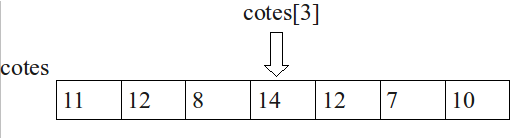
\includegraphics[width=0.8\linewidth,height=0.8\textheight,keepaspectratio=true]{/home/clr/Documents/Cours/DEV1Q2/TDTableau/fr/image/tabPres.png}
						\end{center}
                
                    \caption[tabPres.png]{tabPres.png}
                \end{figure}
                    
            \par
        
        Contrairement \`a algo o\`u on a le choix des valeurs desbornes pour les indices, 
        en Java, les indices varient de \verb@0@ \`a \verb@taille du tableau - 1@.
      
            \par
        0 est l'indice de d\'epart.
            \par
        
			
		\subparagraph{D\'eclaration et cr\'eation : 2 \'etapes} 
		
					\textcolor{white}{.} \par
				
        En Java, l'\'etape de cr\'eation est s\'epar\'ee de l'\'etape de d\'eclaration. \par
				
        En effet, l'\'etape de d\'eclaration r\'eserve un emplacement m\'emoire sur la pile qui contiendra une adresse 
        o\`u trouver la valeur des \'el\'ements du tableau. 
        La cr\'eation connaitra lataille du tableau, le cr\'eera sur le tas et remplira l'adresse sur la pile.
      
            \par
        \begin{figure}[hbt]
				    \begin{center}
					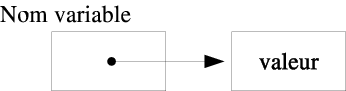
\includegraphics[width=0.8\linewidth,height=0.8\textheight,keepaspectratio=true]{/home/clr/Documents/Cours/DEV1Q2/TDTableau/fr/image/reference.png}
						\end{center}
                
                    \caption[reference.png]{reference.png}
                \end{figure}
                    
            \par
        
			
		\subparagraph{D\'eclaration} 
		
					\textcolor{white}{.} \par
				
        Pour d\'eclarer un tableau : 
      
            \par
        \begin{verbatim}
Type[] identifier
      \end{verbatim}
        Par exemple :\par
				\verb@int []@ est le type tableau d'entiers\par
				\verb@String []@ est le type tableau de chaines de caract\`eres
      
            \par
        \begin{verbatim}
int [] cotes ;
String [] noms;
      \end{verbatim}
			
		\subparagraph{Cr\'eation} 
		
					\textcolor{white}{.} \par
				
        Pour cr\'eer un tableau : 
      
            \par
        \begin{verbatim}
identifier = new Type[taille]
      \end{verbatim}
        Par exemple :\par
				\verb@new int[3]@\par
				\verb@new String[taille]@ o\`u \verb@taille@ est d\'efini
      
            \par
        \begin{verbatim}
int [] entiers ; // déclaration
entiers = new int[3]; // création
      \end{verbatim}
        La d\'eclaration et la cr\'eation peuvent \^etre combin\'ees
      
            \par
        \begin{verbatim}
int [] entiers = new int[3];
      \end{verbatim}
			
		\subparagraph{Initialisation} 
		
					\textcolor{white}{.} \par
				
        Par d\'efaut, les \'el\'ements sont initialis\'es \`a 0 (num\'eriques) ou false (bool\'eens).
        Ce ne sont pas forc\'ement les valeurs initiales que nous d\'esirons. Pour changer \c ca :
      
            \par
        \begin{verbatim}
identifier = new Type[] {x, x}
      \end{verbatim}
        Par exemple :\par
				\verb@new int[] {42, 17, -5}@\par
				\verb@new String[] {"foo", "bar"}@
            \par
        \begin{verbatim}
int [] entiers = new int[] {0x2A, 021, −5};
String [] noms = new String[] {" Victoria ", "Melanie", "Melanie", "Emma", "Geri"};
double[] réels ;
réels = new double[] {4.2, −1};
      \end{verbatim}
			
		\subparagraph{Cas particulier : d\'eclaration, cr\'eation et initialisation} 
		
					\textcolor{white}{.} \par
				
        On peut d\'eclarer le tableau, le cr\'eer et l'initialiser en une seule \'etape, en donnant ses valeurs :
      
            \par
        \begin{verbatim}
int [] entiers = {0x2A, 021, −5};
double[] pseudoRéels = {4.5, 1E−4, −4.12, Math.PI};

// Mais si sur 2 lignes :
double[] réels ;
réels = {4.2, −1}; // FAUX
      \end{verbatim}
			
		\subparagraph{Acc\`es aux \'el\'ements} 
		
					\textcolor{white}{.} \par
				
					\begin{enumerate}
				
			\item 0 est l'indice de d\'epart
			\item les indices varient de 0 \`a taille du tableau - 1
			\item la taille du tableau est son nombre d'\'el\'ements
					\end{enumerate}
				
            \par
        \begin{verbatim}
int [] entiers = {3, 14, 15};
int entier = entiers [2]; // entier vaut 15
entiers [1] = 85;
entier = 0;
entier = entiers [ entier +1]; // entier vaut 85
      \end{verbatim}Par exemple :
            \par
        \begin{verbatim}

package be.heb.esi. lg1 . tutorials . tableaux ;

public class InitialisationTableau {
    public static void main(String [] args) {
      int [] entiers = new int[10];
      for(int i = 0; i < 10; i++) {
        entiers [ i ] = i;
      }
    }
}\end{verbatim}\subsection{Taille logique et physique}
		    Parfois, on connait la taille d'un tableau lorsqu'on \'ecrit l'algorithme (par exemple s'il s'agit
        de retenir les ventes pour les douze mois de l'ann\'ee) mais ce n'est pas toujours le cas (par
        exemple, connait-on le nombre de produits vendus par le magasin ?).
		  
            \par
        
		    Si cette taille n'est pas connue, une possibilit\'e est
        d'attribuer au tableau une taille maximale (sa taille physique) et de retenir dans une
        variable le nombre r\'eel de cases utilis\'ees (sa taille logique).
		  
            \par
        \begin{verbatim}
// Calcule et affiche la quantité vendue de x produits.
module statistiquesVentes()
    cpt : tableau [1 à 1000] d’entiers
    i, numéroProduit, quantité : entiers
    nbArticles : entier
    
    lire nbArticles
    pour i de 1 à nbArticles faire
      cpt[i] ← 0
    fin pour
    
    afficher "Introduisez le numéro du produit :"
    lire numéroProduit
    tant que numéroProduit > 0 ET numéroProduit <= nbArticles faire
      afficher "Introduisez la quantité vendue :"
      lire quantité
      cpt[numéroProduit] ← cpt[numéroProduit] + quantité
      afficher "Introduisez le numéro du produit :"
      lire numéroProduit
    fin tant que
    
    pour i de 1 à nbArticles faire
      afficher "quantité vendue de produit ", i, " : ", cpt[i]
    fin pour
fin module
\end{verbatim}\subsection{Taille d'un tableau en Java}
		    En Java, un tableau connait sa taille
      
            \par
        \begin{verbatim}
identifier.length
      \end{verbatim}\begin{verbatim}
int [] entiers = {4, 5, 6};
int taille = entiers . length ;
System.out. println ( taille ); // écrit 3
      \end{verbatim}Par exemple : 
            \par
        \begin{verbatim}
package be.heb.esi. lg1 . tutorials . tableaux ;

public class SimpleParcoursAscendant {
    public static void main(String [] args){
      int [] entiers = {1, 2, 3, 4, 5, 6, 7, 8, 9, 10};
      for(int i = 0; i < entiers . length ; i = i + 1) {
        System.out. println ( entiers [ i ]);
      }
    }
}
      \end{verbatim}ou encore
            \par
        \begin{verbatim}
package be.heb.esi. lg1 . tutorials . tableaux ;

public class SimpleParcoursDescendant {
    public static void main(String [] args){
      int [] entiers = {1, 2, 3, 4, 5, 6, 7, 8, 9, 10};
      for(int i = entiers . length − 1; i >= 0; i = i−1) {
        System.out. println ( entiers [ i ]);
      }
    }
}
      \end{verbatim}\subsection{Tableau et param\`etres de module}
		    Un tableau peut \^etre pass\'e en param\`etre \`a un module mais qu'en est-il de sa taille ? Il
        serait utile de pouvoir appeler le m\^eme module avec des tableaux de tailles diff\'erentes. Pour
        permettre cela, la taille du tableau re\c cu en param\`etre est d\'eclar\'ee avec une variable (qui
        peut \^etre consid\'er\'e comme un param\`etre entrant).
		  
            \par
        
		    Par exemple :
		  
            \par
        \begin{verbatim}
module afficherTaille(tabEntier↓ : tableau [1 à n] d’entiers)
    afficher "J’ai reçu un tableau de ", n, " éléments".
fin module
      \end{verbatim}
        Ce \verb@n@ va prendre la taille pr\'ecise du tableau utilis\'e \`a chaque appel
        et peut \^etre utilis\'e dans le corps du module. Bien s\^ur il s'agit l\`a de la 
        \textbf{taille physique} du tableau. 
      
            \par
        
        Si une partie seulement du tableau doit \^etre trait\'ee, il convient de \textbf{passer \'egalement
        la taille logique en param\`etre}.
      
            \par
        Par exemple :
            \par
        \begin{verbatim}
module afficherTailles(tabEntiers↓ : tableau [1 à n] d’entiers, tailleLogique : entier)
    afficher "J’ai reçu un tableau rempli de ", tailleLogique, " éléments "
    afficher "sur ", n, " éléments au total."
fin module
      \end{verbatim}
        Un module peut retourner un tableau.
      
            \par
        \begin{verbatim}
// Crée un tableau statique d’entiers de taille 10, l’initialise à 0 et le retourne.
module créerTableau() → tableau [1 à 10] d’entiers
    tab : tableau [1 à 10] d’entiers
    i : entier
    pour i de 1 à 10 faire
      tab[i] ← 0
    fin pour
    retourner tab
fin module

module principalAppelTableau()
    entiers : tableau [1 à 10] d’entiers
    i : entier
    entiers ← créerTableau()
    pour i de 1 à 10 faire
      afficher entiers[i]
    fin pour
fin module
      \end{verbatim}
        Attention, il n'est pas possible de lire ou d'afficher un tableau en une seule instruction ; il faut des
        instructions de lecture ou d'affichage individuelles pour chacun de ses \'el\'ements.
      
            \par
        \subsection{Tableau et param\`etres de m\'ethodes}Un tableau peut \^etre un param\`etre d'une m\'ethode.
            \par
        Par exemple :
            \par
        \begin{verbatim}
public static void afficher ( int [] entiers ) {
    for(int i = 0; i <entiers . length ; i ++) {
      System.out. println ( entiers [ i ]);
    }
}\end{verbatim}L'appel pourrait \^etre
            \par
        \begin{verbatim}
int [] cotes = {12, 8, 10, 14, 9};
afficher ( cotes );
      \end{verbatim}
			
		\subparagraph{Passage de param\`etre par valeur} 
		
					\textcolor{white}{.} \par
				
        En Java, passage de param\`etre par valeur.
        Pour un tableau, cela signifie que l'on ne peut pas
        modifier le tableau dans son ensemble mais que
        l'on pourra modifier ses \'el\'ements.
      
            \par
        Par exemple :
            \par
        \begin{verbatim}
public static void remplir ( int [] entiers , int val ) {
    for(int i = 0; i <entiers . length ; i ++) {
      entiers [ i ] = val;
    }
}\end{verbatim}L'appel pourrait \^etre
            \par
        \begin{verbatim}
int [] cotes = new int[16]; // Ne pas oublier de le créer !
remplir ( cotes , 20 );
      \end{verbatim}MAIS :
            \par
        \begin{verbatim}
public static void méthodeFausse( double[] réels ) {
    double[] réelsDePassage = {4.2, −7, Math.PI};
    réels = réelsDePassage; // INUTILE
}\end{verbatim}
        Quel que soit l'appel, le tableau que l'on passe en
        param\`etre ne sera pas modifi\'e.
      
            \par
        
			
		\subparagraph{Un tableau peut \^etre une valeur de retour} 
		
					\textcolor{white}{.} \par
				
            \par
        Par exemple :
            \par
        \begin{verbatim}
ppublic static int [] créer ( int taille , int val ) {
    int [] entiers = new int[ taille ];
    for(int i = 0; i < taille ; i ++) {
      entiers [ i ] = val;
    }
    return entiers ;
}\end{verbatim}L'appel pourrait \^etre
            \par
        \begin{verbatim}
int [] cotes = créer(16, 20);
      \end{verbatim}\subsection{Parcours d'un tableau \`a une dimension.}
		    Soit le tableau \verb@tab@ d\'eclar\'e ainsi
		  
            \par
        \begin{verbatim}
tab : tableau [1 à n] de T  // où T est un type quelconque
      \end{verbatim}Envisageons d'abord le parcours complet et voyons ensuite les parcours avec arr\^et pr\'ematur\'e.
            \par
        
			
		\subparagraph{Parcours complet.} 
		
					\textcolor{white}{.} \par
				
		    Pour parcourir compl\`etement un tableau, on peut utiliser la boucle 
		    \verb@pour@ comme dans
        l'algorithme suivant o\`u \guillemotleft  traiter \guillemotright  va d\'ependre du probl\`eme concret pos\'e : afficher, modifier,
        sommer, . . .
      
            \par
        \begin{verbatim}
// Parcours complet d’un tableau via une boucle pour
// Les déclarations sont omises pour ne pas alourdir les algorithmes.
pour i de 1 à n faire
    traiter tab[i]
fin pour
      \end{verbatim}
			
		\subparagraph{Parcours avec sortie pr\'ematur\'ee.} 
		
					\textcolor{white}{.} \par
				
        Parfois, on ne doit pas forc\'ement parcourir le tableau jusqu'au bout mais on pourra s'arr\^eter
        pr\'ematur\'ement si une certaine condition est remplie. Par exemple :
        
					\begin{enumerate}
				
			\item on cherche la pr\'esence d'un \'el\'ement et on vient de le trouver ;
			\item on v\'erifie qu'il n'y a pas de 0 et on vient d'en trouver un.
					\end{enumerate}
				
        La premi\`ere \'etape est de transformer le \verb@pour@ 
        en \verb@tant que@ ce qui donne l'algorithme
      
            \par
        \begin{verbatim}
// Parcours complet d’un tableau via une boucle tant-que
i ← 1
tant que i ≤ n faire
    traiter tab[i]
    i ← i+1
fin tant que
		  \end{verbatim}
		    On peut \`a pr\'esent introduire le test d'arr\^et. Une contrainte est qu'on voudra, \`a la fin de la
        boucle, savoir si oui ou non on s'est arr\^et\'e pr\'ematur\'ement et, si c'est le cas, \`a quel indice.
      
            \par
        
        Il existe essentiellement deux solutions, avec ou sans variable bool\'eenne. En g\'en\'eral, la
        solution [A] sera plus claire si le test est court.
		  
            \par
        
			
		\subparagraph{Parcours avec sortie pr\'ematur\'ee sans variable bool\'eenne} 
		
					\textcolor{white}{.} \par
				
            \par
        \begin{verbatim}
// Parcours partiel d’un tableau sans variable booléenne
i ← 1
tant que i ≤ n ET test sur tab[i] dit que on continue faire
    i ← i+1
fin tant que

si i > n alors
    // on est arrivé au bout
sinon
    // arrêt prématuré à l’indice i.
fin si
      \end{verbatim}
        Il faut \^etre attentif \`a \textbf{ne pas inverser les deux parties du test}. 
        Il faut absolument v\'erifier  que l'indice est bon avant de tester la valeur \`a cet indice.
      
            \par
        
        On pourrait inverser les deux branches du si-sinon en inversant le test mais attention \`a ne
        pas tester \verb@tab[i]@ car \verb@i@ n'est peut-\^etre pas valide.
      
            \par
        
        Dans certains cas, le si-sinon peut se simplifier en un simple return d'une condition.
      
            \par
        Par exemple : 
            \par
        \begin{verbatim}
// Indique si un zéro est présent dans le tableau
module contientZéro(tab : tableau [1 à n] d’entiers) → booléen
    i : entier
    i ← 1
    tant que i ≤ n ET tab[i] ≠ 0 faire
      i ← i+1
    fin tant que
    retourner i ≤ n // Si le test est vrai c’est qu’on a trouvé un 0
fin module
      \end{verbatim}
			
		\subparagraph{Parcours avec sortie pr\'ematur\'ee avec variable bool\'eenne} 
		
					\textcolor{white}{.} \par
				
            \par
        \begin{verbatim}
// Parcours partiel d’un tableau avec variable booléenne
i ← 1
trouvé ← faux
tant que i ≤ n ET NON trouvé faire
    si test sur tab[i] dit que on a trouvé alors
      trouvé ← vrai
    sinon
      i ← i+1
    fin si
fin tant que
// tester le booléen pour savoir si arrêt prématuré.
      \end{verbatim}
        Attention \`a bien choisir un nom de bool\'een adapt\'e au probl\`eme et \`a l'initialiser \`a la bonne
        valeur. Par exemple, si la variable s'appelle \guillemotleft  continue \guillemotright 
        
					\begin{enumerate}
				
			\item initialiser la variable \`a vrai ;
			\item le test de la boucle est \guillemotleft  . . .ET continue \guillemotright  ;
			\item mettre la variable \`a faux pour sortir de la boucle.
					\end{enumerate}
				
            \par
        \subsection{Erreurs fr\'equentes et exceptions lanc\'ees en Java}
					\begin{enumerate}
				
			\item \verb@NullPointerException@ : 
            si vous essayez d'acc\'eder \`a un \'el\'ement d'un tableau qui n'a pas \'et\'e cr\'e\'e
            (le tableau vaut null dans ce cas) ;
          
			\item \verb@ArrayIndexOutOfBoundsException@ : 
            si vous donnez un indice qui n'existe pas (ex : tab [10] quand il n'y a que 10 \'el\'ements dans le tableau).
          
					\end{enumerate}
				
            \par
        \section{Exercices}
				Maintenant, mettons tout \c ca en pratique.
      
            \par
        \subsection{Compr\'ehension d'algorithme}
          Pour ces exercices, nous vous demandons de comprendre des algorithmes donn\'es. 
          
			
		\subparagraph{Compr\'ehension} 
		
                \textcolor{white}{.} \par
            
							  Que vont-ils afficher ?
              
					\begin{itemize}
				
			\item \begin{verbatim}
module boucle1 ()
    x : entier
    x ← 0
    tant que x < 12 faire
      x ← x+2
    fin tant que
    afficher x
fin module
				\end{verbatim} \textcolor{gray}{\underline{\hspace*{2em}}} 
			\item \begin{verbatim}
module boucle2 ()
    ok : booléen
    x : entier
    ok ← vrai
    x ← 5
    tant que ok faire
      x ← x+7
      ok ← x MOD 11 ≠ 0
    fin tant que
    afficher x
fin module
				\end{verbatim} \textcolor{gray}{\underline{\hspace*{2em}}} 
			\item \begin{verbatim}
module boucle3 ()
    ok : booléen
    cpt, x : entiers
    x ← 10
    cpt ← 0
    ok ← vrai
    tant que ok ET cpt < 3 faire
      si x MOD 2 = 0 alors
        x ← x+1
        ok ← x < 20
      sinon
        x ← x+3
        cpt ← cpt + 1
      fin si
    fin tant que
    afficher x
fin module
				\end{verbatim} \textcolor{gray}{\underline{\hspace*{2em}}} 
			\item \begin{verbatim}
module boucle4 ()
    pair, grand : booléens
    p, x : entiers
    x ← 1
    p ← 1
    faire
      p ← 2*p
      x ← x+p
      pair ← x MOD 2 = 0
      grand ← x > 15
    jusqu’à ce que pair OU grand
    afficher x
fin module
				\end{verbatim} \textcolor{gray}{\underline{\hspace*{2em}}} 
			\item \begin{verbatim}
module boucle5 ()
    i, x : entiers
    ok : booléen
    x ← 3
    ok ← vrai
    pour i de 1 à 5 faire
      x ← x+i
      ok ← ok ET (x MOD 2 = 0)
    fin pour
    si ok alors
      afficher x
    sinon
      afficher 2 * x
    fin si
fin module
				\end{verbatim} \textcolor{gray}{\underline{\hspace*{2em}}} 
			\item \begin{verbatim}
module boucle6 ()
    i, j, fin : entiers
    pour i de 1 à 3 faire
      fin ← 6 * i - 11
      pour j de 1 à fin par 3 faire
        afficher 10 * i + j
      fin pour
    fin pour
fin module
				\end{verbatim} \textcolor{gray}{\underline{\hspace*{10em}}} 
					\end{itemize}
				
            \par
        \subsection{Compr\'ehension de codes Java}
			
		\subparagraph{Instructions r\'ep\'etitives} 
		
                \textcolor{white}{.} \par
            
							Quelles instructions r\'ep\'etitives sont correctes parmi les suivantes? 
							Expliquez pourquoi les autres ne le sont pas.
						
            \begin{itemize} 
        
            \item[ \ding{"6F} ] proposition 1
							\begin{Java}
While ( condition ) {
	// instructions
}							\end{Java}
        
            \item[ \ding{"6F} ] proposition 2
							\begin{Java}
do while ( condition ) {
	// instructions
}							\end{Java}
        
            \item[ \ding{"6F} ] proposition 3
							\begin{Java}
while ( true ) {
	// instructions
}							\end{Java}
        
            \item[ \ding{"6F} ] proposition 4
							\begin{Java}
while ( true ) do {
	// instructions
}							\end{Java}
        
            \item[ \ding{"6F} ] proposition 5
							\begin{Java}
FOR ( int i=0; i<=10; i=i+2 ) DO {
	// instructions
}							\end{Java}
        
            \item[ \ding{"6F} ] proposition 6
							\begin{Java}
for ( int i=0; i<=10; i=i+2 ) {
	// instructions
}							\end{Java}
        
            \item[ \ding{"6F} ] proposition 7
							\begin{Java}
for ( int i=0; i<=10; i=i+2 ) do {
	// instructions
}							\end{Java}
        
            \item[ \ding{"6F} ] proposition 8
							\begin{Java}
for ( int i=9; i>=0; i=i-2 ) {
	// instructions
}							\end{Java}
        
            \end{itemize} 
        
			
		\subparagraph{Activit\'e 'remplir les blancs'} 
		
                \textcolor{white}{.} \par
            
								Quel op\'erateur de comparaison Java repr\'esente la relation suivante? 
							
            \par
        
					\begin{enumerate}
				
			\item "est \'egal \`a" ?                      \textcolor{gray}{\underline{\hspace*{2em}}} 
			\item "est diff\'erent de" ?                \textcolor{gray}{\underline{\hspace*{2em}}} 
					\end{enumerate}
				
								Quel op\'erateur bool\'een Java repr\'esente l'op\'erateur logique suivant? 
							
            \par
        
					\begin{enumerate}
				
			\item le ET :   \textcolor{gray}{\underline{\hspace*{2em}}} 
			\item le OU :   \textcolor{gray}{\underline{\hspace*{2em}}} 
			\item le NON :  \textcolor{gray}{\underline{\hspace*{1em}}} 
					\end{enumerate}
				
			
		\subparagraph{Exp\'erience} 
		
					\textcolor{white}{.} \par
				
					Indiquez l'affichage obtenu par ce code.
				
            \par
        
			
		\subparagraph{Compr\'ehension} 
		
                \textcolor{white}{.} \par
            
							  Que vont-ils afficher ?
              \begin{Java}
public class Boucles {

	public static void main ( String[] args ) {
		int facteur;
		final int VALEUR = 3;
	
		for (facteur = 1 ; facteur <= 10 ; facteur++){		
			System.out.print(facteur*VALEUR+" ");
		}
		System.out.println();
	}
}			\end{Java} \textcolor{gray}{\underline{\hspace*{16em}}} 
			
		\subparagraph{Exercice Tant que} 
		
					\textcolor{white}{.} \par
				
					\'Ecrivez en Java l'algorithme suivant.
				
            \par
        \begin{verbatim}
MODULE Test

    nb, produit : Entier
    produit ← 1 

    LIRE nb
    TANT QUE nb ≠ 0 FAIRE
        produit ← produit * nb
        LIRE nb 
    FIN TANT QUE
    AFFICHER produit
    
FIN MODULE
			    \end{verbatim}
			
		\subparagraph{Exercice Pour} 
		
					\textcolor{white}{.} \par
				
					\'Ecrivez en Java l'algorithme suivant.
				
            \par
        \begin{verbatim}
MODULE Test

    nb: Entier
    i : Entier

    LIRE nb
    POUR i DE 1 A nb FAIRE
        AFFICHER i
    FIN POUR

FIN MODULE
			     \end{verbatim}\subsection{\`A vous de jouer...}
          Il est temps de se lancer et d'\'ecrire vos premiers modules et programmes Java correspondant. 
          Voici quelques conseils pour vous guider dans la r\'esolution de tels probl\`emes :
          
					\begin{itemize}
				
			\item il convient d'abord de bien comprendre le probl\`eme pos\'e ; assurez-vous qu'il est parfaitement sp\'ecifi\'e ;
			\item d\'eclarez ensuite les variables (et leur type) qui interviennent dans l'algorithme ; les noms des variables risquant de ne pas \^etre suffisamment explicites ;
			\item \textbf{mettez en \'evidence les variables \guillemotleft  donn\'ees \guillemotright , les variables \guillemotleft  r\'esultats \guillemotright  et les variables de travail ;}
			\item n'h\'esitez pas \`a faire une \'ebauche de r\'esolution en fran\c cais avant d'\'elaborer l'algorithme d\'efinitif pseudo-cod\'e.
			\item \'Ecrivez la partie algorithmique \textbf{AVANT} de vous lancer dans la programmation en Java.
					\end{itemize}
				
            \par
        
        \'Ecrivez les algorithmes et codez les programmes Java correspondant qui 
          
					\begin{enumerate}
				
			\item re\c coit un naturel \verb@n@ et affiche
              
					\begin{enumerate}
				
			\item les \verb@n@ premiers entiers strictement positifs ;
			\item les \verb@n@ premiers entiers strictement positifs en ordre d\'ecroissant ;
			\item les \verb@n@ premiers carr\'es parfaits ;
			\item les \verb@n@ premiers naturels impairs ;
			\item les naturels impairs qui sont inf\'erieurs ou \'egaux \`a \verb@n@.
					\end{enumerate}
				
              Si le \verb@n@ re\c cu n'est pas strictement positif, votre programme s'arr\^etera en g\'en\'erant une erreur/une exception.
            
			\item 
              demande \`a l'utilisateur d'introduire un entier positif (non strictement). 
              Ce module permet \`a l'utilisateur de se tromper \`a plusieurs reprises mais l'utilisateur devra donner
              une bonne valeur pour arr\^eter le programme.
              (On suppose tout de m\^eme que l'utilisateur ne donne que des valeurs enti\`eres !) 
            
			\item 
              lit une s\'erie de nombres entiers positifs, jusqu'\`a ce que l'utilisateur
              encode la valeur 0. Les nombres multiples de 3 seront affich\'es au fur et \`a mesure et le nombre
              de ces multiples sera affich\'e en fin de traitement.
              
            \par
        
              Pensez \`a utiliser le module \'ecrit ci-dessus qui permet de lire un entier positif.
              
            \par
        
			\item 
              retourne la somme des chiffres qui forment un nombre naturel \verb@n@
              Attention, on donne au d\'epart le nombre et pas ses chiffres. Exemple : 133045 doit donner
              comme r\'esultat 16, car 1 + 3 + 3 + 0 + 4 + 5 = 16.
            
			\item 
              lit une suite de nombres positifs entr\'es au clavier et affiche
              le maximum, le minimum, leur somme et la moyenne. \par
				
              La fin de la suite de nombre sera signifi\'ee par une valeur sentinelle que vous choisirez
              judicieusement.
            
			\item 
              v\'erifie si un entier donn\'e forme un palindrome ou non. Un nombre
              palindrome est un nombre qui lu dans un sens (de gauche \`a droite) est identique au nombre
              lu dans l'autre sens (de droite \`a gauche). Par exemple, 1047401 est un nombre palindrome.
            
			\item 
                affiche les \verb@n@ premiers termes de la suite suivante : 
                \verb@1, –1, 2, –3, 5, –8, 13, –21, 34, –55, …@
                o\`u \verb@n@ est un entier strictement positif re\c cu en param\`etre.\par
				
                Si le \verb@n@ re\c cu n'est pas strictement positif, votre programme s'arr\^etera en g\'en\'erant une erreur/une exception.
            
					\end{enumerate}
				
            \par
        En java, n'oubliez pas d'\'ecrire la javadoc et la m\'ethode main pour tester vos m\'ethodes.
            \par
        
			
		\subparagraph{Jeu de la fourchette} 
		
					\textcolor{white}{.} \par
				
          \'Ecrivez un algorithme qui simule le jeu de la fourchette. Ce jeu consiste \`a essayer de d\'ecouvrir
          un nombre quelconque compris entre 0 et 100 inclus, tir\'e au sort par l'ordinateur (la primitive
          \verb@hasard(n : entier)@ retourne un entier entre 0 inclus et n exclus). \par
				
          L'utilisateur a droit \`a huit essais maximum.\par
				
          \`A chaque essai, l'algorithme devra afficher un message indicatif
          
					\begin{itemize}
				
			\item \guillemotleft  nombre donn\'e trop petit \guillemotright 
			\item ou \guillemotleft  nombre donn\'e trop grand \guillemotright . 
					\end{itemize}
				
          En conclusion, 
          
					\begin{itemize}
				
			\item soit \guillemotleft  bravo, vous avez trouv\'e en [nombre] essai(s) \guillemotright 
			\item soit \guillemotleft  d\'esol\'e, le nombre \'etait [valeur] \guillemotright .
					\end{itemize}
				
            \par
        \'Ecrivez le code java correspondant.
            \par
        
        Aide en Java : un petit tour dans l'API de la classe Random devrait vous aider \`a trouver l'\'equivalent du
        \verb@hasard(n : entier)@ en Java
    
            \par
        
				\end{document}
			